\documentclass[a4paper, 10pt]{article}

\usepackage{times}

\usepackage{cite}

\usepackage{placeins}

\usepackage{graphicx}
\graphicspath{{images/}}

\usepackage{amsmath}

\title{\huge Platform for Anomaly Detection in Time-Series}

\begin{document}

\maketitle

\noindent \hrulefill

\small
\textit{
Abstract: The goal of this paper is to present a platform that integrates a number of functionalities necessary in the process of anomaly detection, from preprocessing towards various anomaly detection techniques and visualization methods. The purpose of this tool is to allow a developer to test, select and fine tune different algorithms that best fit anomaly detection in a given domain. To demonstrate the utility of the platform, we present a series of experiments done with different methods for anomaly detection on time-series and evaluate their results.
}

\noindent \hrulefill

\textit{
Keywords: Anomaly Detection, time-series
}

\normalsize

\section{Introduction}

We rely on computer and automation systems to manage complex tasks. They are used in many fields and have many applications. Computer systems are used in industrial, academic, commercial and financial applications because of their speed and reliability. Because a defect in such a system can lead to large monetary loss and potentially even loss of life, we need systems that monitor other systems. These systems need to be able to detect faults and anomalous behavior in some way. Algorithms that detect anomalous behavior are therefore necessary and important.

Other applications of anomaly detecting systems include systems that monitor our health. We would like to identify as soon as possible the onset of any disease. By monitoring our health we may be able to spot individuals that have a high risk of contracting some disease and allow medical professionals to act in time to improve their quality of life.

Most anomaly detection algorithms were developed for a given problem or a given range of problems. While creating general algorithms is really hard and may not even be possible, it is best to try many different approaches. The problem we are trying to solve is the lack of a designated platform or tool that can aid in deciding which anomaly detection algorithm works best for a particular problem.

In this paper we propose a platform that enables a user to test a variety of anomaly detection algorithms, with emphasis on time series data. This data has the form $X = \{x_t \in {\rm I\!R} : \forall t \ge 0\}$. Furthermore, we will use the following functional definition of what an anomaly is: An anomaly is a data point or set of data, which is significantly different from all other data points or sets. This means that in order to define an anomaly, one must first have a notion of nominal data. The term anomaly is relative and can not be applied to a data-point independently of any dataset.

The following chapters are structured as follows: In Section \ref{relwork} we describe previous and related work on the subject. Next, in Section \ref{platform} we give a brief description of the developed platform and its features. In Section \ref{methods} we describe the types of anomaly detection methods provided by our platform. We will test these methods in Section \ref{experiments}. This will be followed by a discussion on the future research directions and implications in Section \ref{discussion}.

\section{Related Work \label{relwork}}

Most methods for anomaly detection are developed for a given field or have a specific application. In \cite{nnfd1994} and \cite{MMAD2006} the authors developed methods to detect anomalies in airplane data. In \cite{ghad2018} similar methods were developed for IoT. In \cite{ADDSCIL} methods for detecting anomalies in Big Data are presented. In \cite{NDTSDII1996} methods are used to detect anomalies in industrial machinery.

In \cite{outlierSurvey2014} a host of algorithms and techniques are described and categorized. The authors found that while some algorithms in different fields are very similar, most algorithms are hard to generalize. They also note, that numerous formulations of anomaly detection problems are not sufficiently explored, i.e. it is not known how well some algorithms perform in a field that was not intended for that algorithm.

Efforts to bundle up different anomaly detection algorithms have already begun. In \cite{egads2015} the authors introduced an open source, generic framework for detecting anomalies in large scale time-series data.

In \cite{tpad2018} a platform is proposed, that offers tools for data visualization, filtering and classification for a variety of data formats, including but not limited to time series data.

We believe that there is a real advantage in a platform that offers a variety of anomaly detection methods to the user. One can test the performance of a number of anomaly detection algorithms for some given test data. By having as many implementations of these algorithms as possible, the user can easily test as many algorithms as she wants with minimal effort and cost.

\section{The Platform \label{platform}}
 
In this section we present the anomaly detection platform and its functionalities for time-series data. In Figure \ref{fig:workflow} the envisioned workflow is presented. 

\subsection{Data Loading}

The user starts by loading in some data that she wishes to analyze. Because data can be stored in many different formats, the platform was designed to work with excel, Comma Separated Values (CSV) and Attribute-Relation File Format (ARFF) files, alongside MAT files. 

\subsection{Plotting}

The user can choose to visualize the data using the visualization tools provided by the platform. We provide tools both for time-series and non time-series data. For time-series data we provide tools for plotting, histograms and Fourier decomposition.

\subsection{Preprocessing}

The user can apply transformations to the dataset either to smooth out the data in an attempt to improve the classification results. For this we provide high-pass, low-pass and band-pass filters. We call this step preprocessing.

\subsection{Anomaly Detection}

Next, a user can try out a host of anomaly detection algorithms. Each one will have a set of parameters. These can be fine tuned to improve the classification quality. The quality of the classification can be measured using classification metrics. The confusion matrix can be generated as well as some derived metrics such as precision and recall.

When the user is satisfied with the classification, she can use the parameters of the classification method either for future tests or to implement a specialized system for monitoring anomalies.

In the next chapter we present the types of anomalies together with the detection methods used to detect them.

\begin{figure}
\centering
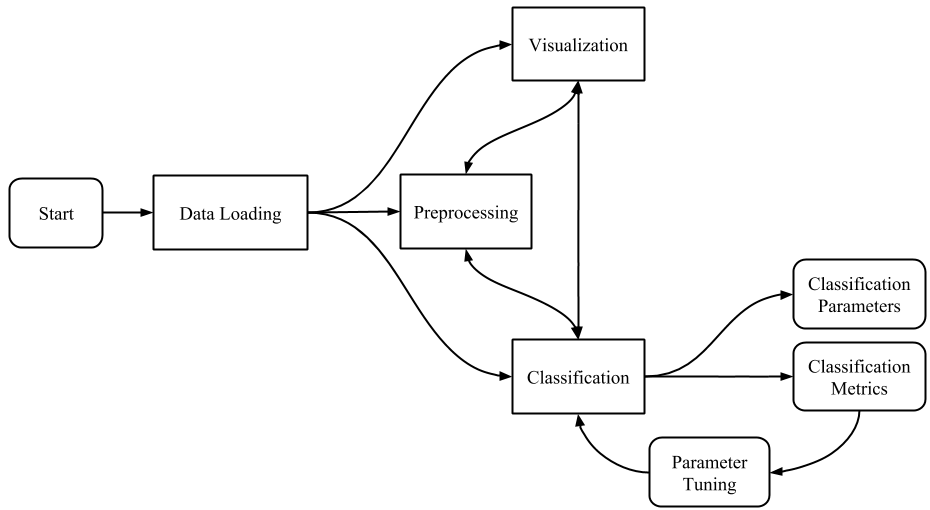
\includegraphics[width=0.7\textwidth]{Workflow}
\caption{Workflow of the classification process.}
\label{fig:workflow}
\end{figure}

\FloatBarrier

\section{Anomaly Detection Techniques \label{methods}}

In this section we give short descriptions of some of the possible anomaly types. For each anomaly type we present some methods for detecting such an anomaly. \\

In principle anomaly detection is similar to system identification. We would like to have a model of the system working in the ``nominal'' state. In the artificial intelligence fields it can be considered as a classification problem, since we assign labels to data.

Anomaly detection is slightly different from these in one regard: anomalies are generally rare, and comprise a very small percent of the data. Some detection methods go for the system identification route, and try to find a model that best fits the nominal data, as well as excludes the anomalous points. Some methods go for the classification route, where artificial intelligence methodologies are used for classification. 

The problem is that the quality of classification provided by the above mentioned methods depend on the size of the dataset. The essence of anomaly detection lies in the fact, that anomalies are rare events, and most datapoints in the training data are ``nominal'' points. 

Some datasets do not even contain anomalies, and algorithms are expected to learn the nominal functioning of the system from ``clean data''. We call a dataset that doesn't contain anomalies a clean dataset. \\

Another classification can be whether or not the methods are online or offline methods. Offline methods usually perform better, since for each data point we can use both past and future values. These methods may be applied in batch, or can be used online, but the detection will have a delay. \\

Given these constraints one can start to classify the anomaly types and detection algorithms.

\subsection{Outliers}

The first type of problem is concerned with classifying each element as anomalous or nominal. We define a function $label$ that labels a data-point $x \in X$ either as anomalous or nominal:
$$c_x = label(x,X)$$
$$c_x \in \{Nominal, Anomaly\}$$


\subsubsection{Bounded Method}

One might be able to label elements as anomalies by setting global lower and upper bounds. This can be used to detect obvious anomalies such as extreme temperature levels or very high blood pressure. 

In the platform we provide a method that classifies a point as an anomaly if it is outside certain bounds. This can be done even with any derivative of the function. We call this \emph{Bounded Derivative Method}. BDM is defined as:
$$
	BDM(x) = 
	\begin{cases}
       \text{Nominal} & \text{if } B^+ > f(x)^{(n)} > B^-\\
    	\text{Anomaly} & \text{otherwise}
    \end{cases}
$$

where $B^+$ and $B^-$ are the upper and lower bounds, and $f(x)^{(n)}$ is the $n$-th derivative of the signal. An example of the usage can be seen in Figure \ref{fig:BDM}.

\begin{figure}
\centering
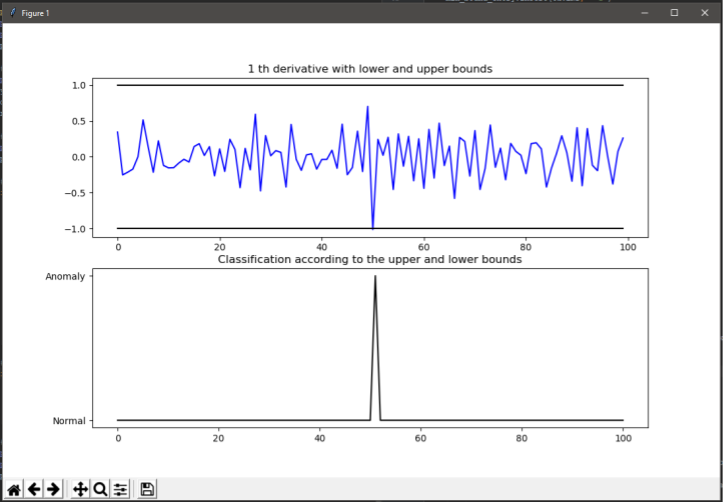
\includegraphics[width=0.7\textwidth]{BDM}
\caption{A signal with a higher than average disturbance in the middle is detected by the method. Forward difference is used as an approximation for the derivative.}
\label{fig:BDM}
\end{figure}

\FloatBarrier

Even though this detection is trivial, it can be used to detect many types of anomalies. This is because of the fact that anomalies appear outside normal working conditions.

\subsubsection{Model Distance Method}

If such a predicate function is not possible, a more complex approach can be used.\\

Since the time-series is generated by a generative process, one could hope to be able to accurately describe the underlying process, and create a model of the system:
$$x_t^* = f(t)$$
where $x_t^*$ is the predicted value of $x$ at time $t$. \\

Given such a model, one can label the anomalies based on some threshold given a dstance metric $d: X \times X \rightarrow {\rm I\!R}$. If the distance between the predicted value $x_t^*$ and the actual value $x_t$ is greater than some threshold $d_{max}$, $x_t$ can be considered an anomaly:
$$
    p(x_t) =
        \begin{cases}
            \text{Anomaly} & \text{if } d(x_t, f(t)) \ge d_{max} \\
            \text{Nominal} & \text{otherwise}
        \end{cases}
$$

Although such a model is highly useful, sometimes in practice it is good enough to consider only the neighboring points. For illustration we will use a method inspired from \cite{MMAD2006}. This method is known as the \emph{Double Sided Median Method} for anomaly detection. By using a sliding window, we calculate the mean of the values inside the window, and if a given value is outside the allowed bounds, it is considered an anomaly. 

$$
	DSMM(x_t) = 
		\begin{cases}
            \text{Anomaly} & \text{if } |f(x_t) - mean(f(x_{t-k}), \dots, f(x_{t+k}))| > d \\
            \text{Nominal} & \text{otherwise}
        \end{cases}
$$

An example can be seen in Figure \ref{fig:DSMM}. \\

\begin{figure}
\centering
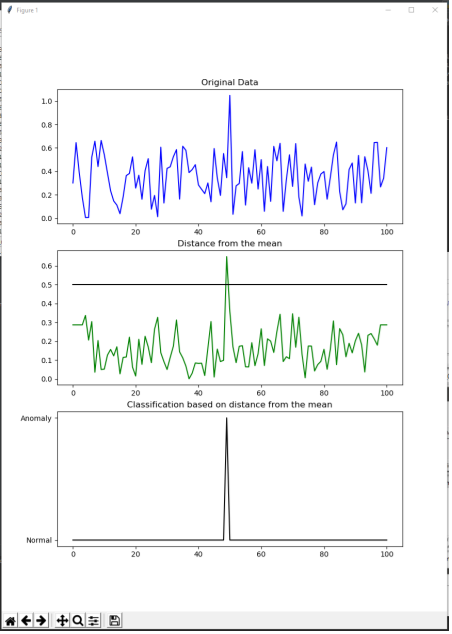
\includegraphics[width=0.49\textwidth]{DSMM}
\caption{In the top figure, we can see the raw signal. In green we see the distance of each point from the mean of the sliding window. The black line from the middle plot is the distance limit. If the values falls outside the maximum distance, that point is considered to be an anomaly, as can be seen in the bottom plot.}
\label{fig:DSMM}
\end{figure}

\FloatBarrier

\subsubsection{Linear Approximation Method}

TODO

\subsubsection{Autoregressive Method}

Other regressive models, that use the past values to predict the new values are also used: $x_t^* = f(x_{t-1}, x_{t-2}, \dots, x_{t-n}), n \ge 1$. If given that the data starts at $t=0$ and $t-n > 0$, we use a sliding window approach, where we generate a prediction for the next value based on the actual old values. This is useful if we can model the time series using an auto-regressive model.

\subsection{Change Point Detection}

Change Point detection focuses on the underlying model of the process. The data is generated by a generative process $f(t, p)$, where $p \in {\rm I\!R}^n$ are the parameters of the model. That process is considered to be the nominal generative process. There is also an error $e(t)$ associated with the process. The error function is usually considered to be white noise.
$$x_t = f(t, p) - e(t)$$

This detection methods focuses on more long term changes compared to regular outlier detection methods. When a change in the system behavior is observed, it is considered an anomalous behavior. In other words, we constantly update the parameters of the process $p_n$, and compare it with the previous parameters $p_{n-1}$. $p_n$ is considered an anomalous behavior if $|p_n - p_{n-1}| > d_p$, where $d_p \in {\rm I\!R}$ is a threshold value.

An example of this is illustrated in Figure \ref{fig:changepoint}.

\begin{figure}
\centering
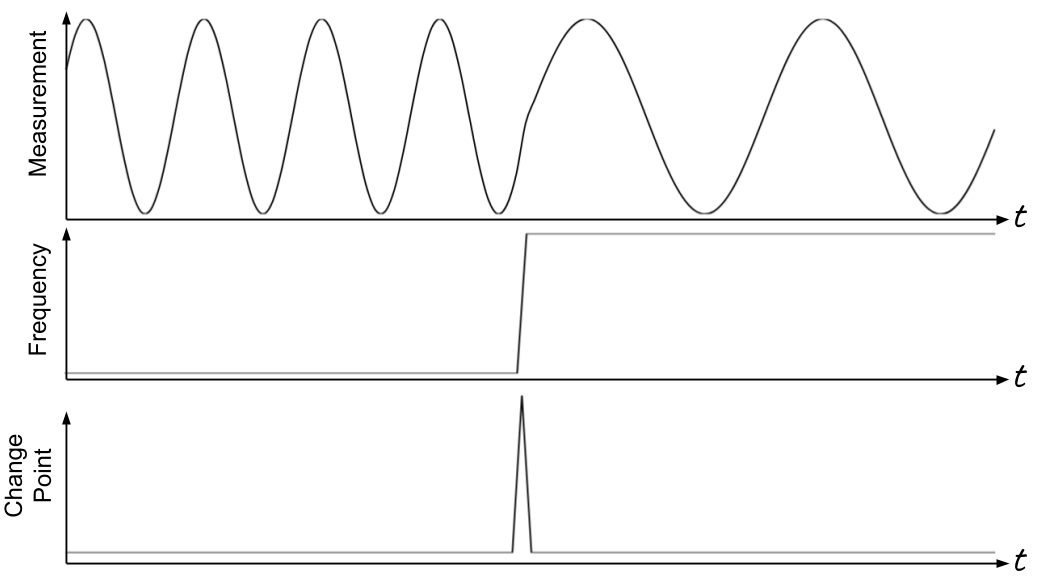
\includegraphics[width=0.7\textwidth]{ChangePoint}   
\caption{In the top most graph, we can see the observed process. In this case it is a pure sine wave. In the middle graphs we can see the coefficient of the model, which in this case is just a function of it's frequency, since it is enough to perfectly describe the process. We consider as anomaly either the change point, either all the points where the model is outside some bounds.}
\label{fig:changepoint}
\end{figure}

\section{Experiments \label{experiments}}

In this section we will compare a number of anomaly detection methods, and compare their results. \\

We will use precision and recall to compare the methodologies presented.

First dataset

\begin{figure}
\centering
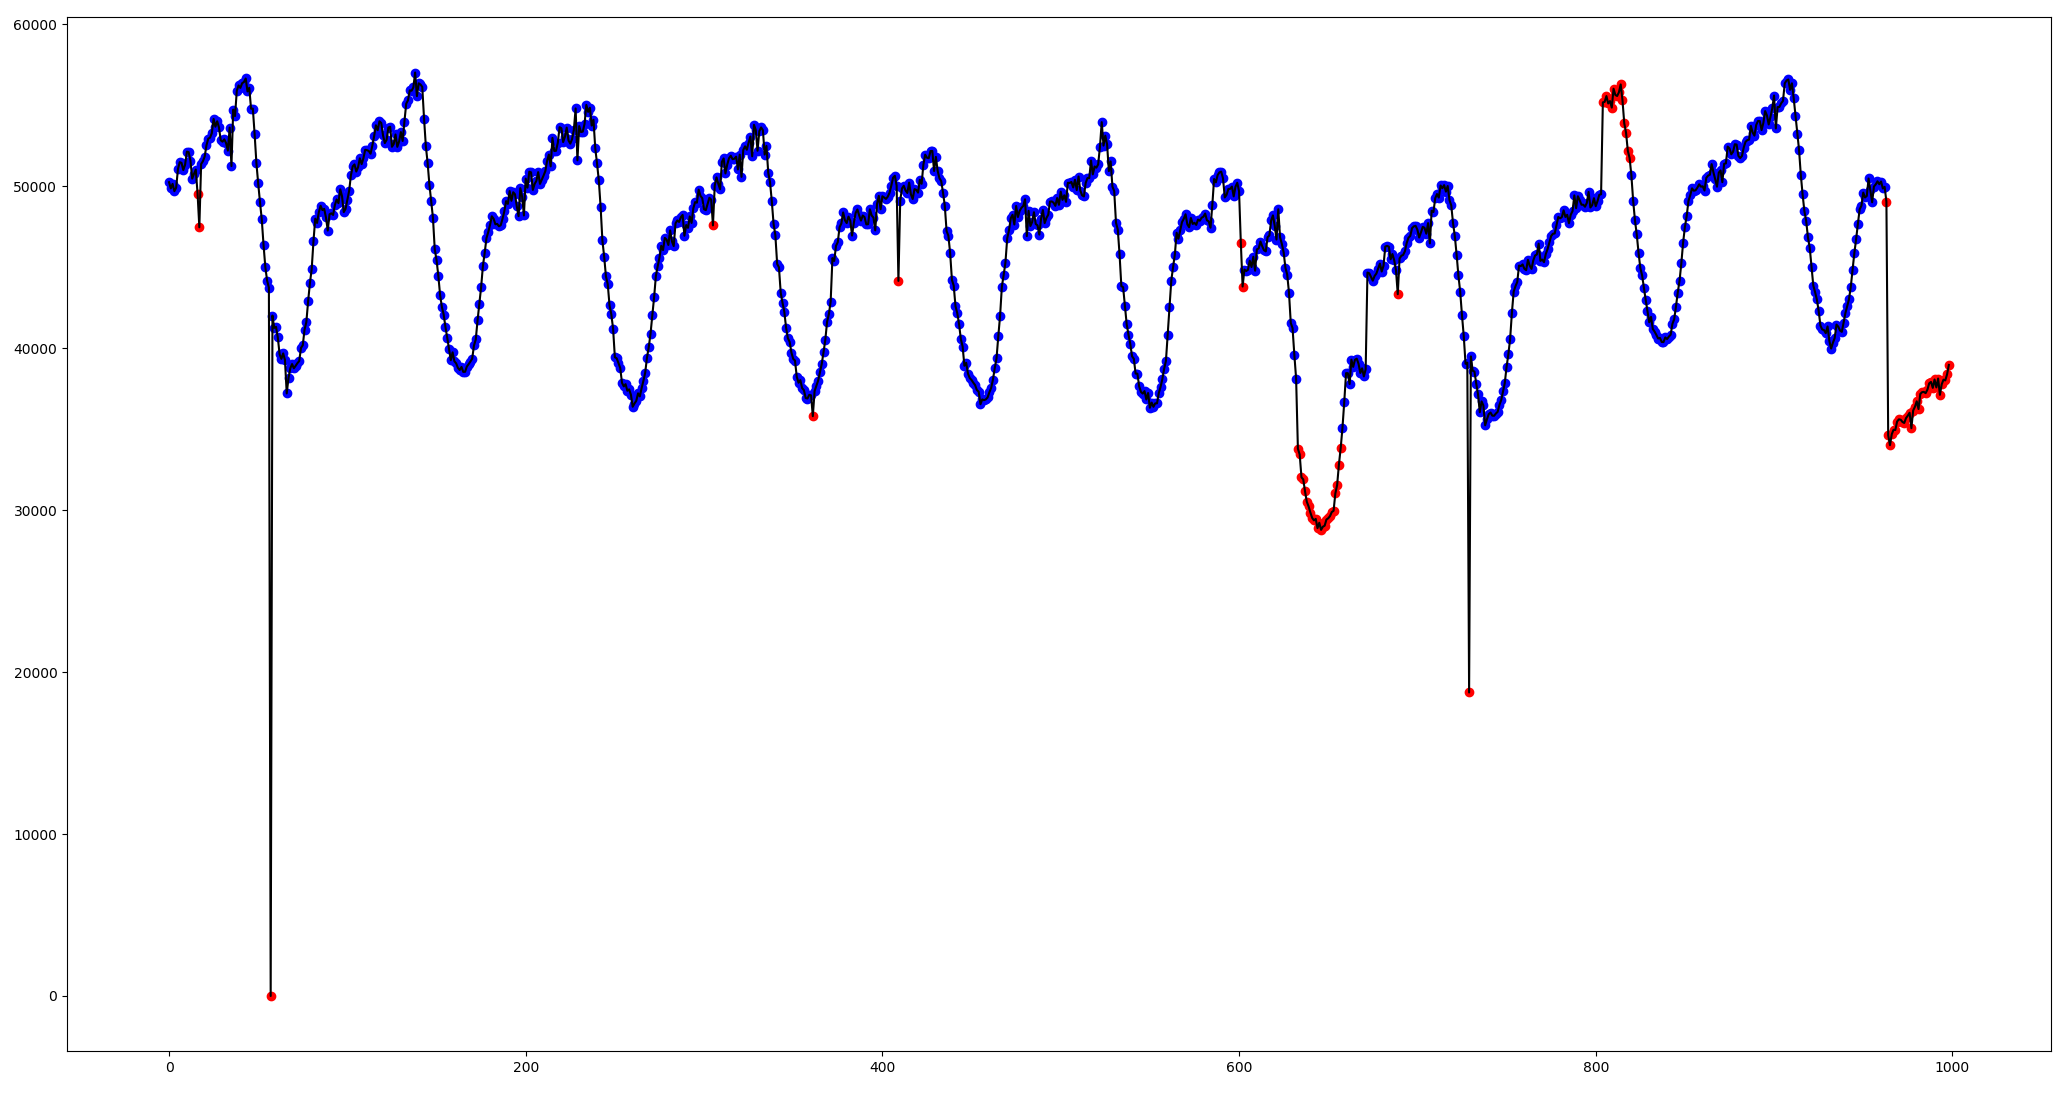
\includegraphics[width=0.7\textwidth]{testplot1}   
\caption{Description pending.}
\label{fig:test1}
\end{figure}

\FloatBarrier

\begin{center}
\begin{tabular}{| c | c | c |}
\hline
Method                      & Precision & Recall \\ \hline
Bounded Derrivative (d = 0) & 1         & 0.3678 \\ \hline
Bounded Derrivative (d = 1) & 0.6       & 0.0689 \\ \hline
Median Method               & 0.33      & 0.0919 \\ \hline
\end{tabular}
\end{center}

\section{Discussion \label{discussion}}

As a conclusion, we think it is a good idea to pull together all the anomaly detection methods used for time-series into a single platform.

\bibliography{refs} 
\bibliographystyle{ieeetr}

\end{document}
